% =========================
% main.tex (Overleaf-ready)
% =========================
\documentclass[11pt]{article}

% ---------- Page / Font ----------
\usepackage[margin=1in]{geometry}

% ---------- Math ----------
\usepackage{amsmath, amssymb, amsthm, mathtools, bm}

% ---------- Algorithms ----------
\usepackage[ruled,vlined]{algorithm2e}

% ---------- Figures and Table ----------
\usepackage{graphicx}
\usepackage{subcaption}
\usepackage{booktabs} % 提供三线表支持 (\toprule, \midrule, \bottomrule, \cmidrule)
\usepackage{multirow} % 提供跨行合并单元格的支持 (\multirow)
% \usepackage{graphicx} % 提供缩放表格的支持 (\resizebox)
\usepackage{float}
\graphicspath{{images/}} % IMPORTANT: figures folder path

% ---------- Citations ----------
\usepackage[numbers, sort&compress]{natbib} % compatible with many DL venues; use \citet, \citep

% ---------- Links ----------
\usepackage[colorlinks=true,linkcolor=blue,citecolor=blue,urlcolor=blue]{hyperref}
\usepackage{authblk}

% =========================
% Environment Definitions
% =========================
% --- 环境定义 ---
% 1. 定义定理样式 (可选，Plain是默认的斜体内容，Definition通常是正体)
\theoremstyle{definition} 
\newtheorem{definition}{Definition}

% 2. 定义 Remark 样式 (通常标题斜体，内容正体)
\theoremstyle{remark}
\newtheorem{remark}{Remark}

% 3. 定义 Theorem 样式 (标题加粗，内容斜体)
\theoremstyle{plain}
\newtheorem{theorem}{Theorem}
\newtheorem{lemma}{Lemma}

% =========================
% SciML Macros
% =========================
\newcommand{\mL}{\mathcal{L}}           % Loss
\newcommand{\Ncal}{\mathcal{N}}        % Neighbors
\newcommand{\R}{\mathbb{R}}            % Real numbers
\newtheorem{proposition}{Proposition} % Proposition

% Partial derivative: \pd[2]{u}{x} -> \frac{\partial^2 u}{\partial x^2}
\newcommand{\pd}[3][]{%
  \frac{\partial^{#1} #2}{\partial #3^{#1}}%
}

% Optional: common operators / notation
\DeclareMathOperator{\diver}{div}
\DeclareMathOperator{\grad}{grad}

\title{G-GRN: A Graph-based Neural Operator for Elliptic PDEs with Discontinuous Coefficients}

\author[1]{Shuxuan Liang\thanks{Email: \href{mailto:shuxuan0228@hanyang.ac.kr}{shuxuan0228@hanyang.ac.kr}}}
\author[1]{Gwanghyun Jo\thanks{Corresponding author. Email: \href{mailto:gwanghyun@hanyang.ac.kr}{gwanghyun@hanyang.ac.kr}}}

\affil[1]{Department of Applied Mathematics, Hanyang University}


\setlength{\affilsep}{1em}

\date{\today}

\begin{document}
\maketitle

\begin{abstract}
We present G-GRN (Graph-based Generalized Regression Network), a physics-informed graph neural network that replaces automatic differentiation with precomputed Generalized Finite Difference (GFD) stencil coefficients as fixed message-passing weights to solve 2D elliptic interface problems with discontinuous coefficients. Because derivative accuracy depends on stencil order rather than network smoothness, G-GRN benefits from mesh refinement where standard Physics-Informed Neural Networks (PINNs) stagnate. Training minimizes a $\beta$-normalized strong-form loss enforcing the governing PDE, boundary conditions, and both interface transmission conditions. On three interface geometries (circular, oscillating, elliptic) with coefficient contrasts up to $1{:}100$, G-GRN reduces the relative $L^2$ error by $1.7\times$ and training time by $2.5\times$ over a standard PINN at resolution $N=64$, with accuracy robust to the contrast magnitude and a convergence order ($p=0.54$) more than twice that of the PINN ($p=0.24$).
\end{abstract}

\section{Introduction}
\label{sec:introduction}

Elliptic interface problems, partial differential equations of the form $-\nabla\cdot(\beta\nabla u) = f$ with piecewise-constant coefficients, are fundamental to computational science and engineering. They model physical systems where material properties change sharply across an internal boundary $\Gamma$: composite materials with mismatched stiffness, immiscible fluid interfaces, and biological membranes separating distinct tissue regions \cite{peskin2002immersed, leveque1994immersed}. Without special treatment at $\Gamma$, convergence rates of standard numerical schemes deteriorate, because the coefficient jump forces a gradient discontinuity that smooth basis functions cannot capture \cite{babuvska1970finite, li2006immersed}.

Restoring accuracy requires methods that explicitly encode the jump in $\beta$. While the finite element method can achieve high-order convergence on interface-conforming meshes, generating such meshes becomes expensive for complex or moving interfaces \cite{babuvska1970finite}. Fixed-grid approaches avoid this cost by modifying difference stencils near $\Gamma$ to enforce the jump conditions; the Immersed Interface Method (IIM) \cite{leveque1994immersed} and the Matched Interface and Boundary (MIB) method \cite{zhou2006fictitious} follow this strategy with increasing accuracy. Generalized Finite Differences (GFD) go further, abandoning structured grids altogether and reconstructing derivative operators from arbitrary node distributions via weighted least-squares \cite{liszka1980finite, benito2001influence}.

These methods, however, share a reliance on hand-crafted stencils that must be redesigned for each new interface geometry. Physics-Informed Neural Networks (PINNs) \citep{raissi2019physics} sidestep this constraint by embedding PDE residuals directly into the loss function of a neural network, requiring neither stencils nor mesh conformity. The framework has been applied successfully to forward and inverse problems alike \citep{karniadakis2021physics, lu2021deepxde}, but interface problems expose its weaknesses. Multilayer perceptrons are biased toward low-frequency solutions \cite{rahaman2019spectral}, making it difficult to resolve the sharp gradients that arise at $\Gamma$. Multi-term losses (PDE residual, boundary conditions, interface jumps) compete for gradient magnitude, often destabilizing training \cite{wang2021understanding}; in some configurations, the network fails to converge entirely \cite{krishnapriyan2021characterizing}. Domain decomposition \cite{jagtap2020conservative}, discontinuity-aware architectures \cite{hu2022discontinuity}, and axis-augmented formulations for imperfect contact conditions \cite{oh2025physics} offer partial remedies at the cost of additional complexity. In preliminary experiments, we observed a more fundamental limitation: when we refined the grid from $N=24$ to $N=32$, the PINN's error did not decrease, suggesting that autograd-computed derivatives cannot capitalize on finer spatial discretizations.

Graph Neural Networks (GNNs) \cite{kipf2016semi, hamilton2017inductive} offer a natural alternative for PDE problems on unstructured domains, since their message-passing operations \cite{gilmer2017neural} directly encode the topology of the computational mesh. In physics simulation, graph-based models have learned complex dynamics from mesh-level interactions \cite{sanchez2020learning, pfaff2020learning}, and message passing has been applied directly to PDE solution operators \cite{brandstetter2022message}. Yet none of these approaches exploit the derivative information that classical numerical stencils can provide. GFD stencils encode precise local gradient structure; GNNs offer flexible nonlinear approximation on graphs. The possibility of combining these two capabilities, using precomputed stencil coefficients as message-passing weights, remains unexplored.

We propose G-GRN (Graph-based Generalized Regression Network) to fill this gap. G-GRN treats precomputed GFD stencil coefficients as edge weights in a graph neural network, replacing autograd with scatter-based derivative approximation. Because derivative accuracy now depends on stencil order rather than network smoothness, the method naturally benefits from mesh refinement, a property that standard PINNs lack. Training minimizes a strong-form loss combining the PDE residual, Dirichlet boundary conditions, and both interface transmission conditions ($[u]$ and $[\beta\partial_n u]$), with Fourier feature encoding \cite{tancik2020fourier} to counteract the spectral bias of the underlying MLP. Experiments on three interface geometries (circular, oscillating, elliptic) confirm that G-GRN outperforms standard PINNs in both accuracy and training speed.

The remainder of this paper is organized as follows. Section \ref{sec:problem} formulates the elliptic interface problem. Section \ref{sec:method} details the G-GRN architecture, including graph construction, GFD stencil computation, the network design, and the training protocol. Section \ref{sec:experiments} presents numerical experiments on three test cases, and Section \ref{sec:conclusion} concludes with a discussion of limitations and future directions.

% ==================================================================
% SECTION 2: 题目 (物理与数学定义)
% ==================================================================
\section{Problem Formulation}
\label{sec:problem}

This section formulates the elliptic interface problem studied throughout the paper. Let $\Omega \subset \mathbb{R}^2$ be a bounded computational domain bisected by a closed interface $\Gamma$ into an interior subdomain $\Omega^-$ and an exterior subdomain $\Omega^+$. In $\Omega^- \cup \Omega^+$, the scalar field $u(\mathbf{x})$ satisfies the steady-state diffusion equation:
\begin{equation}
    -\nabla \cdot (\beta(\mathbf{x}) \nabla u(\mathbf{x})) = f(\mathbf{x}),
\end{equation}
where $f(\mathbf{x})$ is a prescribed source term. The diffusion coefficient $\beta(\mathbf{x})$ is piecewise constant with a jump across $\Gamma$:

\begin{equation}
    \beta(\mathbf{x}) =
    \begin{cases}
        \beta^- & \text{for } \mathbf{x} \in \Omega^-, \\
        \beta^+ & \text{for } \mathbf{x} \in \Omega^+,
    \end{cases}
\end{equation}
where $\beta^-$ and $\beta^+$ are strictly positive constants. This discontinuity reduces the regularity of the exact solution: standard finite difference \cite{liszka1980finite} and finite element \cite{babuvska1970finite} methods lose accuracy near $\Gamma$ unless the mesh conforms to the interface geometry.

Well-posedness requires two transmission conditions across $\Gamma$. Let $\mathbf{n}$ denote the unit normal pointing from $\Omega^-$ to $\Omega^+$. The first condition prescribes the jump in the solution value:
\begin{equation}
    [u]_\Gamma \coloneqq u^+|_\Gamma - u^-|_\Gamma = g_1,
\end{equation}
and the second prescribes the jump in the normal flux:
\begin{equation}
    \left[\beta \frac{\partial u}{\partial n}\right]_\Gamma \coloneqq \beta^+ \nabla u^+ \cdot \mathbf{n} - \beta^- \nabla u^- \cdot \mathbf{n} = g_2,
\end{equation}
where $u^\pm$ denote the one-sided limits from $\Omega^\pm$. In many physical settings $g_1 = g_2 = 0$ (perfect contact). When the contrast ratio $\beta^+/\beta^-$ is large, the flux condition forces an abrupt change in $\nabla u$ across $\Gamma$, producing a gradient discontinuity that is difficult to approximate with smooth basis functions.

On the outer boundary $\partial\Omega$ we impose Dirichlet data $u = g_D$. The interface $\Gamma$ is represented implicitly by a level-set function $\phi(\mathbf{x})$ with $\phi < 0$ in $\Omega^-$, $\phi > 0$ in $\Omega^+$, and $\Gamma = \{\mathbf{x} : \phi(\mathbf{x}) = 0\}$. This representation provides a direct formula for the interface normal, $\mathbf{n} = \nabla\phi / |\nabla\phi|$. The combination of discontinuous coefficients, transmission conditions, and the resulting gradient singularity at $\Gamma$ defines the core difficulty of the elliptic interface problem. Section \ref{sec:method} introduces the G-GRN architecture designed to address these challenges. 

% ==================================================================
% SECTION 3: 方法论 (你的核心贡献)
% ==================================================================
\section{Methodology}
\label{sec:method}

In this section, we present the G-GRN framework. The overall pipeline involves constructing a topology-aware graph, precomputing physics-based stencils, and training a neural operator to minimize the residual loss.

% ===================== Graph Construction ======================
\subsection{Graph Construction}
\label{sec:graph_construction}

We represent the computational domain as a graph $\mathcal{G} = (\mathcal{V}, \mathcal{E})$, where the node set $\mathcal{V} = \{\mathbf{p}_i\}_{i=1}^{N}$ combines a uniform background grid with targeted refinement along the interface. First, a Cartesian grid of resolution $n \times n$ is generated to cover the computational domain $\Omega = [-1,1]^2$. Second, to resolve the sharp transition near the discontinuity, we add concentric rings of nodes on both sides of the interface. For each layer $l = 1, \ldots, L_r$, we place $N_\Gamma$ nodes uniformly in the angular direction at radii $R \pm \delta_l$, where the offset is
\begin{equation}
    \delta_l = \frac{w}{2} \cdot \frac{l}{L_r},
\end{equation}
and $w$ is the width of the refinement band. In our default setting, $L_r = 2$, $N_\Gamma = 64$, and $w = 0.1$, producing four rings of 64 nodes within a band of width $0.1$ centered on $\Gamma$. The final node set is the union of the grid nodes and the refinement nodes. Each node $i$ carries a feature vector $\mathbf{v}_i = [x_i, y_i, \phi_i, z_i]^\top \in \mathbb{R}^4$, where $\phi_i$ is the level-set value and $z_i = \text{sgn}(\phi_i) \in \{-1, 1\}$ is the region indicator.

Once the nodes are placed, we establish connectivity via a spatial radius search. An edge exists between node $i$ and node $j$ if their Euclidean distance is less than a cutoff radius $r_c$, excluding self-loops. This radius must be large enough to provide at least 5 neighbors per node for quadratic GFD fitting. We set $r_c = 4.5 / n$, where $n$ is the grid resolution. Since the background spacing is $h = 2/n$ on the domain $[-1,1]^2$, this gives $r_c \approx 2.25 h$, which typically yields 15--25 neighbors for interior nodes.

Treating all edges uniformly is insufficient for interface problems, so we partition $\mathcal{E}$ into two disjoint subsets based on the region indicator. \textit{Homophilous edges} connect nodes within the same subdomain ($z_i = z_j$); they represent connectivity within a continuous medium and are used exclusively for GFD stencil aggregation. \textit{Heterophilous edges} connect nodes across the interface ($z_i \neq z_j$); because differentiation across the discontinuity is ill-posed, these edges instead carry the interface jump constraints. This partition is encoded in a binary edge attribute $e_{ij} \in \{0, 1\}$ that guides the message-passing mechanism. The combination of dense near-interface sampling and explicit edge classification provides the spatial resolution needed to evaluate flux jumps accurately where the solution is least smooth.

% ============================= GFD =============================
\subsection{Generalized Finite Difference Stencils}
\label{sec:gfd}

Evaluating the PDE residual requires accurate spatial derivatives on an unstructured node set. We use the Generalized Finite Difference (GFD) method \cite{liszka1980finite, benito2001influence}, which reconstructs differential operators from arbitrary node distributions by solving a local Weighted Least Squares (WLS) problem. Consider an interior node $i$ at position $\mathbf{p}_i$ and its homophilous neighbors $\mathcal{N}(i)$. Assuming the solution $u$ is locally smooth ($u \in C^2$), the second-order Taylor expansion for a neighbor $j$ is:
\begin{equation}
    u_j \approx u_i + \Delta x_j u_x|_i + \Delta y_j u_y|_i + \frac{\Delta x_j^2}{2} u_{xx}|_i + \Delta x_j \Delta y_j u_{xy}|_i + \frac{\Delta y_j^2}{2} u_{yy}|_i,
\end{equation}
where $\Delta x_j = x_j - x_i$ and $\Delta y_j = y_j - y_i$. To solve for the derivatives, we construct a linear system that minimizes the weighted approximation error. Let $\mathbf{q}_j = [\Delta x_j, \Delta y_j, \frac{1}{2}\Delta x_j^2, \Delta x_j \Delta y_j, \frac{1}{2}\Delta y_j^2]^\top$ be the geometric basis vector. We define the system matrix $\mathbf{V}$, the weight matrix $\mathbf{W}$, and the unknown derivative vector $\mathbf{d}$ as:
\begin{equation}
    \mathbf{V} = [\mathbf{q}_1, \dots, \mathbf{q}_k]^\top, \quad
    \mathbf{W} = \text{diag}(w_1, \dots, w_k), \quad
    \mathbf{d} = [u_x, u_y, u_{xx}, u_{xy}, u_{yy}]^\top,
\end{equation} 
where $\boldsymbol{\delta} = [\delta u_1, \dots, \delta u_k]^\top$ represents the finite differences. The weights $w_j = \phi(\|\mathbf{p}_j - \mathbf{p}_i\|)$ are determined by a decaying kernel function $\phi$ (e.g., Gaussian) to prioritize closer neighbors. The optimal derivatives are obtained by solving the normal equations:
\begin{equation}
    \mathbf{d} = (\mathbf{V}^\top \mathbf{W}^2 \mathbf{V})^{-1} \mathbf{V}^\top \mathbf{W}^2 \boldsymbol{\delta}.
\end{equation}
This yields the derivatives as weighted sums of neighbor differences. For instance, the discrete Laplacian weights $w_{ij}^{\Delta}$ are derived from the rows corresponding to $u_{xx}$ and $u_{yy}$ in the pseudo-inverse matrix $\mathbf{V}^+_{\mathbf{W}} = (\mathbf{V}^\top \mathbf{W}^2 \mathbf{V})^{-1} \mathbf{V}^\top \mathbf{W}^2$.

We theoretically characterize the approximation accuracy of this scheme.
\begin{proposition}[Consistency of GFD Stencil]
\label{prop:consistency}
Let $h = \max_{j \in \mathcal{N}(i)} \|\mathbf{p}_j - \mathbf{p}_i\|$ be the local characteristic length. Assuming the node distribution ensures that $\mathbf{V}^\top \mathbf{W}^2 \mathbf{V}$ is invertible, the GFD approximation is consistent. The local truncation error for second-order derivatives scales as $\mathcal{O}(h)$ for general irregular stencils and improves to $\mathcal{O}(h^2)$ for symmetric neighbor distributions.
\end{proposition}

However, irregular node distributions can lead to numerical instability. We employ an \textit{adaptive order strategy} based on the condition number $\kappa(\mathbf{V}) = \sigma_{\max}(\mathbf{V}) / \sigma_{\min}(\mathbf{V})$, where $\sigma$ denotes the singular values. If $\kappa(\mathbf{V})$ exceeds a stability threshold (e.g., $10^3$) or if the node has insufficient neighbors ($k < 5$), we automatically fall back to a first-order approximation by truncating the basis to linear terms only. This ensures robust gradient estimation even in degenerate geometric configurations.

Stencils are restricted to homophilous edges ($z_i = z_j$) to satisfy the $C^2$ continuity assumption of the Taylor expansion; physics across the interface is handled separately by the jump conditions. The stencil coefficients are precomputed once before training. At each training step, the PDE residual reduces to a sparse matrix-vector product on the GPU:
\begin{equation}
    \mathcal{R}(\mathbf{u}^{(t)}) = \mathbf{L} \mathbf{u}^{(t)} - \mathbf{f},
\end{equation}
where $\mathbf{L} \in \mathbb{R}^{N \times N}$ is the sparse Laplacian matrix assembled from $w_{ij}^{\Delta}$. This operation maps directly to optimized sparse kernels (e.g., \texttt{torch.sparse.mm}).

% ================== Network Architecture ==================
\subsection{Network Architecture}
\label{sec:architecture}

The G-GRN architecture approximates the solution operator by embedding the discretized differential structure into the neural message passing. Figure~\ref{fig:architecture} illustrates the complete training pipeline: from graph construction and feature assignment, through the G-GRN processor layers, to the physics-informed loss evaluation.

\begin{figure}[t]
    \centering
    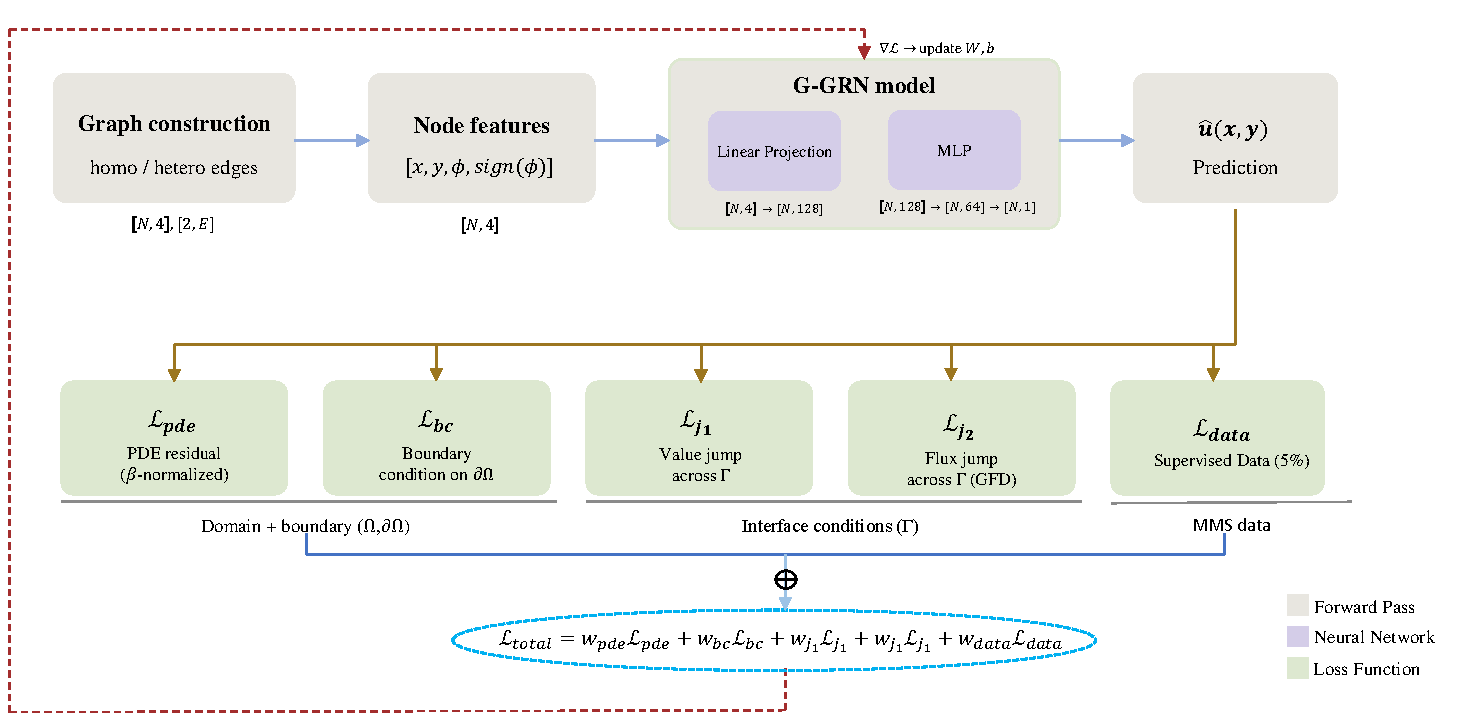
\includegraphics[width=\linewidth]{images/model-struc.pdf}
    \caption{Complete training pipeline for the G-GRN method solving elliptic interface problems $-\nabla \cdot (\beta \nabla u) = f$ with discontinuous $\beta$ across interface $\Gamma$. The graph is constructed with radius based connectivity (homo / hetero edges). Node features are projected through a linear layer and decoded via an MLP. Four physics-informed loss terms enforce the PDE residual, boundary conditions, and the two interface transmission conditions, with derivatives computed via precomputed GFD stencils.}
    \label{fig:architecture}
\end{figure}

The network takes as input the node feature $\mathbf{v}_i \in \mathbb{R}^4$ defined in Section~\ref{sec:graph_construction}. The first G-GRN layer maps $\mathbf{v}_i$ from $\mathbb{R}^4$ to the hidden dimension $\mathbb{R}^H$ without a separate encoding stage; the derivative aggregation within each layer (described below) supplies gradient and curvature information, reducing the need for explicit frequency encoding at the input.

The core computation takes place in $L$ stacked G-GRN layers. Unlike standard graph convolution layers that learn abstract edge weights, our layer explicitly aggregates features to approximate differential operators. In layer $\ell$, for each node $i$, we compute the gradient and Laplacian of the current feature $\mathbf{h}_i^{(\ell)}$ using the frozen GFD stencils over homophilous neighbors:
\begin{equation}
    \mathcal{D}[\mathbf{h}^{(\ell)}]_i = \sum_{j \in \mathcal{N}_{homo}(i)} w_{ij}^{\mathcal{D}} (\mathbf{h}_j^{(\ell)} - \mathbf{h}_i^{(\ell)}), \quad \text{for } \mathcal{D} \in \{ \partial_x, \partial_y, \Delta \}.
\end{equation}
These derivative features are concatenated with the node's state to form a physics-informed context vector $\mathbf{c}_i = [\mathbf{h}_i^{(\ell)}, \nabla \mathbf{h}_i^{(\ell)}, \Delta \mathbf{h}_i^{(\ell)}] \in \mathbb{R}^{4C}$, where $C$ denotes the hidden dimension. This vector is processed by a three-layer MLP that progressively reduces the dimension ($4C \to 2C \to C \to C$), with Layer Normalization and GELU activation after each of the first two linear layers, followed by a residual connection:
\begin{align}
    \mathbf{z}_1 &= \text{GELU}\bigl(\text{LN}(\mathbf{W}_1 \mathbf{c}_i)\bigr), \notag \\
    \mathbf{z}_2 &= \text{GELU}\bigl(\text{LN}(\mathbf{W}_2 \mathbf{z}_1)\bigr), \\
    \mathbf{h}_i^{(\ell+1)} &= \mathbf{h}_i^{(\ell)} + \mathbf{W}_3 \mathbf{z}_2, \notag
\end{align}
where $\mathbf{W}_1 \in \mathbb{R}^{2C \times 4C}$, $\mathbf{W}_2 \in \mathbb{R}^{C \times 2C}$, and $\mathbf{W}_3 \in \mathbb{R}^{C \times C}$.
This design mirrors a learnable numerical scheme: the network observes the local Taylor expansion (via derivatives) and learns a nonlinear correction to evolve the solution.

After $L$ layers, a shallow MLP decoder maps the final embeddings to the scalar prediction $\hat{u}$. The derivative aggregation is parallelized through the \texttt{scatter\_add} primitive: treating $w_{ij}^{\mathcal{D}}(\mathbf{h}_j - \mathbf{h}_i)$ as a directional message, the stencil application reduces to a sparse matrix-matrix multiplication that scales linearly with the number of edges. This design enforces a separation of concerns: the fixed GFD stencils encode the \textit{geometry} (irregular mesh, stencil weights), while the learnable parameters capture the \textit{physics} (solution structure), freeing the network from learning basic discretization rules.

%========================== Loss Formulation =====================================
\subsection{Physics-Informed Loss Formulation}
\label{sec:loss}

Training is driven by a composite loss function that enforces the governing PDE, boundary conditions, and interface constraints. Let $\hat{u}_\theta$ denote the network prediction. We optimize the parameters $\theta$ by minimizing a total loss $\mathcal{L}$:
\begin{equation}
    \mathcal{L}(\theta) = \lambda_{\text{pde}} \mathcal{L}_{\text{pde}} + \lambda_{\text{bc}} \mathcal{L}_{\text{bc}} + \lambda_{\Gamma} (\mathcal{L}_{J_1} + \mathcal{L}_{J_2}),
\end{equation}
where $\lambda_{\text{pde}}, \lambda_{\text{bc}}, \lambda_{\Gamma}$ are hyperparameters balancing the individual objectives.

The first component addresses the governing equation. Standard PINN formulations \cite{raissi2019physics} typically minimize the residual $r = \| -\nabla \cdot (\beta \nabla \hat{u}) - f \|^2$. However, in high-contrast media where the ratio $\beta^+ / \beta^-$ is large (e.g., $10^2$ to $10^3$), this standard form leads to \textit{gradient pathology} \cite{wang2021understanding}. The loss landscape becomes dominated by the high-$\beta$ subdomain, causing the optimizer to neglect the low-$\beta$ region. To mitigate this stiffness, we employ a normalized strong form loss. By dividing the governing equation by $\beta(\mathbf{x})$, we minimize:
\begin{equation}
    \mathcal{L}_{\text{pde}} = \frac{1}{|\mathcal{V}_{\text{int}}|} \sum_{i \in \mathcal{V}_{\text{int}}} \left\| -\Delta \hat{u}_i - \frac{f_i}{\beta_i} \right\|^2.
\end{equation}
Here, the Laplacian $\Delta \hat{u}_i$ is computed via the GFD stencils derived in Section~\ref{sec:gfd}. This normalization acts as a preconditioner, balancing the gradient magnitudes from different material phases to accelerate convergence.

The transmission conditions are enforced explicitly on heterophilous edges $\mathcal{E}_{\text{hetero}}$ that cross the interface, rather than through continuous approximations. Since graph edges are directed and may traverse the interface from $\Omega^-$ to $\Omega^+$ or vice versa, we rely on the destination region indicator $z_j \in \{-1, +1\}$ to ensure consistent orientation. The discrete jump losses for value ($J_1$) and flux ($J_2$) are formulated as:
\begin{align}
    \mathcal{L}_{J_1} &= \frac{1}{|\mathcal{E}_{\text{hetero}}|} \sum_{(i,j) \in \mathcal{E}_{\text{hetero}}} \| z_j (\hat{u}_j - \hat{u}_i) - g_{1,ij} \|^2, \\
    \mathcal{L}_{J_2} &= \frac{1}{|\mathcal{E}_{\text{hetero}}|} \sum_{(i,j) \in \mathcal{E}_{\text{hetero}}} \| z_j (\beta_j \nabla \hat{u}_j \cdot \mathbf{n}_{ij} - \beta_i \nabla \hat{u}_i \cdot \mathbf{n}_{ij}) - g_{2,ij} \|^2.
\end{align}
The factor $z_j$ guarantees that the difference term always represents the canonical jump $[u] = u^+ - u^-$. To ensure high-order geometric accuracy, the interface normal $\mathbf{n}_{ij}$ is evaluated at the edge midpoint $\mathbf{x}_{mid} = (\mathbf{x}_i + \mathbf{x}_j)/2$ using the level-set gradient.

Dirichlet boundary conditions are imposed softly via $\mathcal{L}_{\text{bc}} = \frac{1}{|\mathcal{V}_{\text{bd}}|} \sum \| \hat{u}_i - g_D \|^2$. In our default configuration, we set $\lambda_{\text{pde}} = 1$, $\lambda_{\text{bc}} = 200$, and $\lambda_{\Gamma} = 10$. The implementation also allows independent weights for the value jump ($\lambda_{J_1}$) and flux jump ($\lambda_{J_2}$); when not specified, both default to $\lambda_{\Gamma}$.

%==============================================================================
\subsection{Training Protocols \& Optimization Strategy}
\label{sec:training}

Training physics-informed models requires balancing multiple competing loss terms. We optimize the network parameters using L-BFGS, a quasi-Newton method that approximates inverse Hessian information from recent gradient history. We set the initial learning rate to $\eta_0 = 1.0$, the history size to $50$, and use the strong Wolfe line search condition. This optimizer suits our setting well: the loss is evaluated over a single fixed graph without mini-batching, and the curvature information helps navigate the multi-objective loss landscape. The learning rate follows a cosine annealing schedule \cite{loshchilov2016sgdr}:
\begin{equation}
    \eta(t) = \eta_{\min} + \frac{1}{2}(\eta_0 - \eta_{\min}) \left( 1 + \cos\frac{\pi t}{T} \right),
\end{equation}
where $t$ is the current epoch, $T$ is the total training budget (typically $5 \times 10^3$), and $\eta_{\min} = 10^{-6}$. During training, we track the model state with the lowest error. If the loss diverges to NaN, the best state is restored and training stops early.

% ==================== Experiments ====================
% ================ Numerical Experiments ===========================
\section{Numerical Experiments}
\label{sec:experiments}

Three test problems on the domain $\Omega = [-1,1]^2$ probe different aspects of G-GRN's capability. The first, a circular interface at $R=0.5$, serves as a standard MMS baseline under three coefficient contrasts ($\beta^-/\beta^+ \in \{1/10, \, 1/100, \, 10/1\}$). Example \ref{ex2} introduces angular oscillations into the exact solution, testing whether the method can resolve high-frequency features near $\Gamma$. Example \ref{ex3} replaces the circle with an ellipse ($a=0.6$, $b=0.4$), where the varying normal direction along the interface stresses the flux jump approximation. All three cases admit closed-form solutions, enabling exact error quantification.

All experiments share a common architecture: a 2-layer G-GRN with 128 hidden channels per layer, a depth confirmed sufficient by preliminary ablation. We use L-BFGS (history size 50, strong Wolfe line search) as the optimizer; in our preliminary experiments on these interface problems, L-BFGS converged to consistently lower loss values than Adam. The learning rate follows a cosine annealing schedule from $\eta_0 = 1.0$ to $\eta_{\min} = 10^{-6}$. Four grid resolutions ($N \in \{16, 24, 32, 64\}$) are tested for each example, with Example \ref{ex1} trained for 1\,000 epochs and Examples \ref{ex2}--\ref{ex3} for 2\,000 epochs. The composite loss assigns weights $\lambda_{\text{pde}} = 1$, $\lambda_{\text{bc}} = 200$, and $\lambda_{\Gamma} = 10$; the flux jump term receives a lower weight $w_{J_2} = 0.1$ to suppress noise from stencil-based flux derivatives at coarse resolutions. All computations run on a single NVIDIA RTX PRO 6000 Black Edition GPU.

Prediction accuracy is measured by two norms: the relative $L^2$ error $e_{L^2} = \|u - \hat{u}\|_2 / \|u\|_2$, which quantifies global deviation, and the relative $L^\infty$ error $e_{L^\infty} = \|u - \hat{u}\|_\infty / \|u\|_\infty$, which isolates the worst-case pointwise mismatch. To characterize how these errors decay under grid refinement, we assume a power-law scaling $e_{L^2} \sim C h^p$ with grid spacing $h = 2/(N-1)$ and extract the convergence order $p$ by least-squares regression on $\log h$ versus $\log e_{L^2}$ (Figure \ref{fig:2}).

\begin{figure}
    \centering
    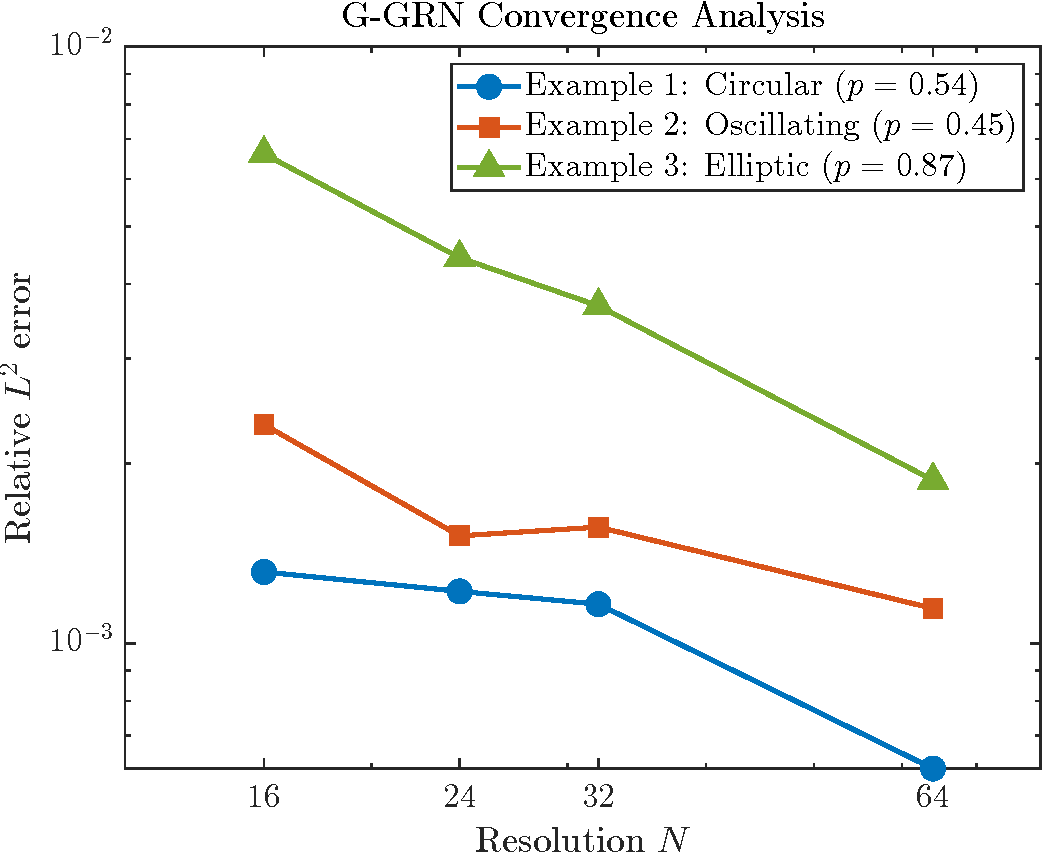
\includegraphics[width=0.5\linewidth]{images/convergence_ggrn.pdf}
    \caption{Convergence of G-GRN across three interface geometries. Log-log plot of relative $L^2$ error versus grid resolution $N$. The fitted slope $p$ denotes the convergence order.}
    \label{fig:2}
\end{figure}

\subsection{Example 1}
For baseline verification, we consider a circular interface $\Gamma: r=R=0.5$. We construct the following piecewise exact solution: \label{ex1}
\begin{equation}
    u(\bf{x}) = \begin{cases}
        r^2, & r < R, \\
        \frac{1}{2} r^2 +1, &r>R.
    \end{cases}
\end{equation}
with $r = x^2 + y^2$. The corresponding source terms are $f = -4 \beta^{-}$ in $\Omega^{-}$ and $f = -2 \beta^{+}$ in $\Omega^{+}$. This solution imposes a value jump $[u] = 1 - \frac{1}{2}r^2$ and a flux jump $[\beta \partial_n u] = (\beta^+ - 2 \beta^{-}) r$ across the interface. We evaluate the method under three coefficient contrasts $\beta^{-}/\beta^{+} \in \{1/10, 1/100, 10/1\}$ and report the MSE, relative $L^2$, relative $L^{\infty}$, and CPU time across four grid resolutions in Table \ref{table1}. At the finest resolution ($N = 64$), the $e_{L^2}$ values for the three contrasts are $6.17 \times 10^{-4}$, $6.80 \times 10^{-4}$, and $7.26 \times 10^{-4}$, respectively; this narrow spread confirms that accuracy is largely insensitive to the magnitude of the coefficient jump, with no significant degradation even at a $1{:}100$ ratio.

\begin{figure}
    \centering
    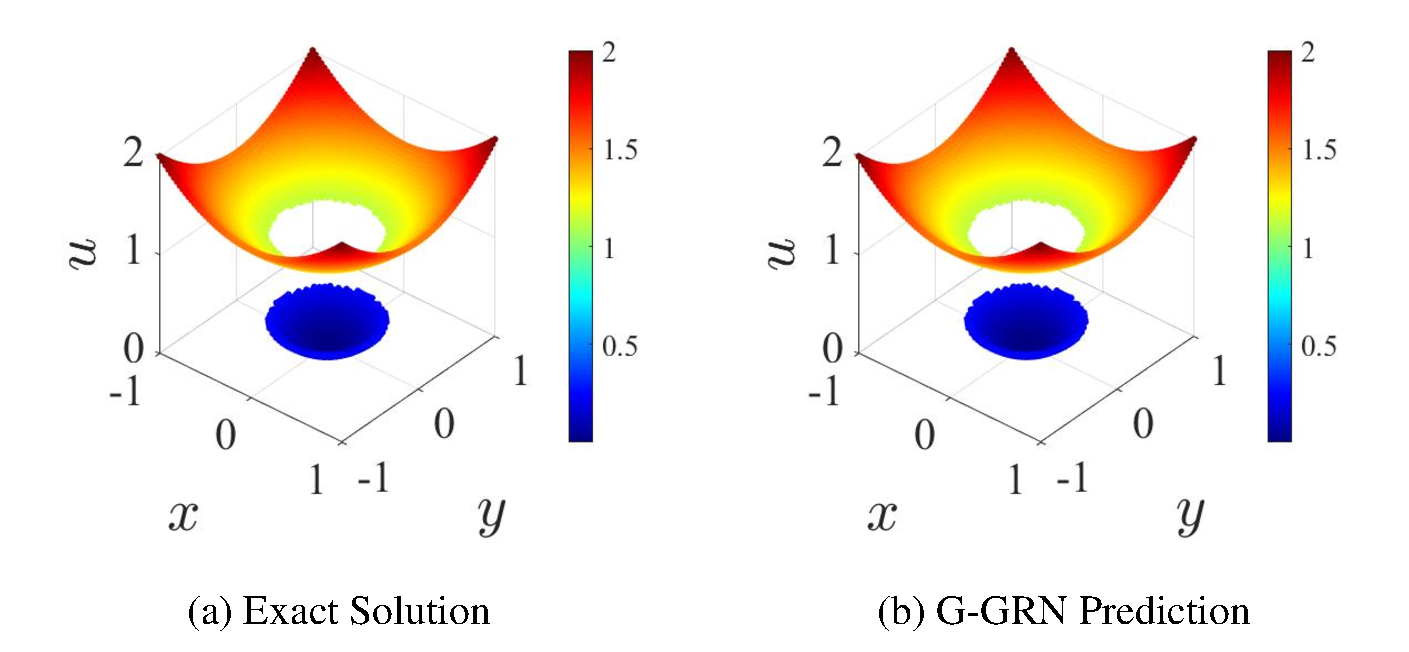
\includegraphics[width=\linewidth]{images/ex1.pdf}
    \caption{Exact Solution vs G-GRN Prediction with setting $(\beta^- / \beta^+) = (1, 10)$ and resolution $N = 64$.}
    \label{fig:ex1_solution}
\end{figure}

\begin{table}[htbp]
    \centering
    \resizebox{\textwidth}{!}{%
    \begin{tabular}{ccccccc}
        \toprule
        \multirow{2}{*}{Layer} & \multirow{2}{*}{$(\beta^-, \beta^+)$} & \multirow{2}{*}{Resolution} & \multicolumn{4}{c}{G-GRN} \\
        \cmidrule(lr){4-7}
        & & & MSE & Rel $L^2$ & Rel $L^\infty$ & CPU Time (s) \\ 
       \midrule
        \multirow{12}{*}{2} 
        & \multirow{4}{*}{(1, 10)} 
        & 16 & 2.12E-06 & 1.32E-03 & 1.26E-03 & 58.97 \\ 
        & & 24 & 2.06E-06 & 1.22E-03 & 1.36E-03 & 49.12 \\ 
        & & 32 & 2.01E-06 & 1.16E-03 & 1.72E-03 & 44.33 \\ 
        & & 64 & 6.02E-07 & \bf{6.17E-04} & 1.45E-03 & 46.26 \\ 
        \cmidrule{2-7}
        & \multirow{4}{*}{(1, 100)} 
        & 16 & 2.17E-06 & 1.33E-03 & 1.19E-03 & 59.86 \\ 
        & & 24 & 2.13E-06 & 1.24E-03 & 1.43E-03 & 48.92 \\ 
        & & 32 & 2.10E-06 & 1.19E-03 & 1.73E-03 & 41.11 \\ 
        & & 64 & 7.32E-07 & \bf{6.80E-04} & 1.14E-03 & 46.52 \\ 
        \cmidrule{2-7}
        & \multirow{4}{*}{(10, 1)} 
        & 16 & 2.37E-06 & 1.39E-03 & 1.31E-03 & 60.72 \\ 
        & & 24 & 2.40E-06 & 1.32E-03 & 1.40E-03 & 45.98 \\ 
        & & 32 & 2.30E-06 & 1.25E-03 & 1.72E-03 & 42.05 \\ 
        & & 64 & 8.34E-07 & \bf{7.26E-04} & 1.40E-03 & 43.21 \\ 
        \bottomrule
    \end{tabular}%
    }
     \caption{The MSE, relative $L^2$, relative $L^\infty$ errors and CPU time of G-GRN method in Example \ref{ex1} where $\beta^{-}/\beta{+} \in \{1/10, 1/100, 10/1\}$.}
    \label{table1}
\end{table}

We compare G-GRN against a standard PINN under identical problem settings (Table \ref{table2}). At $N = 64$ with $\beta^{-}/\beta^{+} = 1/10$, G-GRN achieves $e_{L^2} = 6.17 \times 10^{-4}$, compared to $1.03 \times 10^{-3}$ for the PINN, a $1.7\times$ accuracy gain. Training time also decreases from 114\,s to 46\,s, a $2.5\times$ speedup. Beyond the final accuracy, the two methods differ in their convergence trajectories: the PINN stagnates between $N = 24$ and $N = 32$, with $e_{L^2}$ shifting from $1.41 \times 10^{-3}$ to $1.42 \times 10^{-3}$, while G-GRN maintains a steady error reduction across the entire resolution range. We attribute this contrast to the higher fidelity of GFD-based derivative approximations relative to autograd; the precomputed stencils capture local differential structure more accurately, allowing the network to benefit from each increment in grid resolution.

\begin{table}[htbp]
    \centering
    \resizebox{\textwidth}{!}{%
    \begin{tabular}{ccccccc}
        \toprule
        \multirow{2}{*}{Layer} & \multirow{2}{*}{$(\beta^-, \beta^+)$} & \multirow{2}{*}{Resolution} & \multicolumn{4}{c}{PINN} \\
        \cmidrule(lr){4-7}
        & & & MSE & Rel $L^2$ & Rel $L^\infty$ & CPU Time (s) \\ 
        \midrule
        \multirow{12}{*}{2} 
        & \multirow{4}{*}{(1, 10)} 
        & 16 & 2.52E-06 & 1.44E-03 & 1.66E-03 & 99.00 \\ 
        & & 24 & 2.76E-06 & 1.41E-03 & 1.66E-03 & 99.68 \\ 
        & & 32 & 2.99E-06 & 1.42E-03 & 2.21E-03 & 103.31 \\ 
        & & 64 & 1.67E-06 & \bf{1.03E-03} & 3.03E-03 & 113.62 \\ 
        \cmidrule{2-7}
        & \multirow{4}{*}{(1, 100)} 
        & 16 & 2.49E-06 & 1.43E-03 & 1.74E-03 & 75.28 \\ 
        & & 24 & 2.76E-06 & 1.41E-03 & 1.63E-03 & 87.35 \\ 
        & & 32 & 3.00E-06 & 1.42E-03 & 2.30E-03 & 105.84 \\ 
        & & 64 & 1.53E-06 & \bf{9.85E-04} & 2.86E-03 & 111.25 \\ 
        \cmidrule{2-7}
        & \multirow{4}{*}{(10, 1)} 
        & 16 & 2.44E-06 & 1.41E-03 & 1.81E-03 & 135.95 \\ 
        & & 24 & 2.62E-06 & 1.38E-03 & 1.63E-03 & 98.80 \\ 
        & & 32 & 2.94E-06 & 1.41E-03 & 2.42E-03 & 123.78 \\ 
        & & 64 & 1.63E-06 & \bf{1.01E-03} & 2.83E-03 & 42.83 \\ 
        \bottomrule
    \end{tabular}%
    }
    \caption{Performance of PINN for different values of $(\beta^-, \beta^+)$ at Layer 2.}
    \label{table2}
\end{table}

\subsection{Example 2} \label{ex2}

Example \ref{ex2} tests whether G-GRN can resolve high-frequency spatial features near the interface. Retaining the circular geometry $\Gamma:r = R = 0.5$ from Example \ref{ex1}, we modify the exact solution to include angular oscillations:
\begin{equation}
    u (\bf{x}) = \begin{cases}
        r^2(1 + \epsilon \cos m\theta), &r < R, \\
        \frac{1}{2} ( 1 + \epsilon \cos m\theta) + 1, &r > R.
    \end{cases}
\end{equation}
where $m = 3$, $\epsilon = 0.3$, $\beta^- = 1$, and $\beta^+ = 10$. The resulting source term $f$ acquires a $\cos (m \theta)$ dependence and becomes spatially non-uniform, which increases the angular gradient of the PDE residual near the interface relative to Example \ref{ex1}.

Figure \ref{fig:ex2_solution} shows the exact solution, the G-GRN prediction, and the pointwise absolute error at resolution $N = 64$. The predicted field reproduces the angular oscillation pattern with high fidelity. The error heatmap (Figure \ref{fig:ex2_solution}c) reveals that the largest deviations concentrate near $\Gamma$ at azimuthal angles corresponding to the amplitude peaks of $\cos(3\theta)$, while the interior domain maintains consistently low error levels.

\begin{figure}[t]
    \centering
    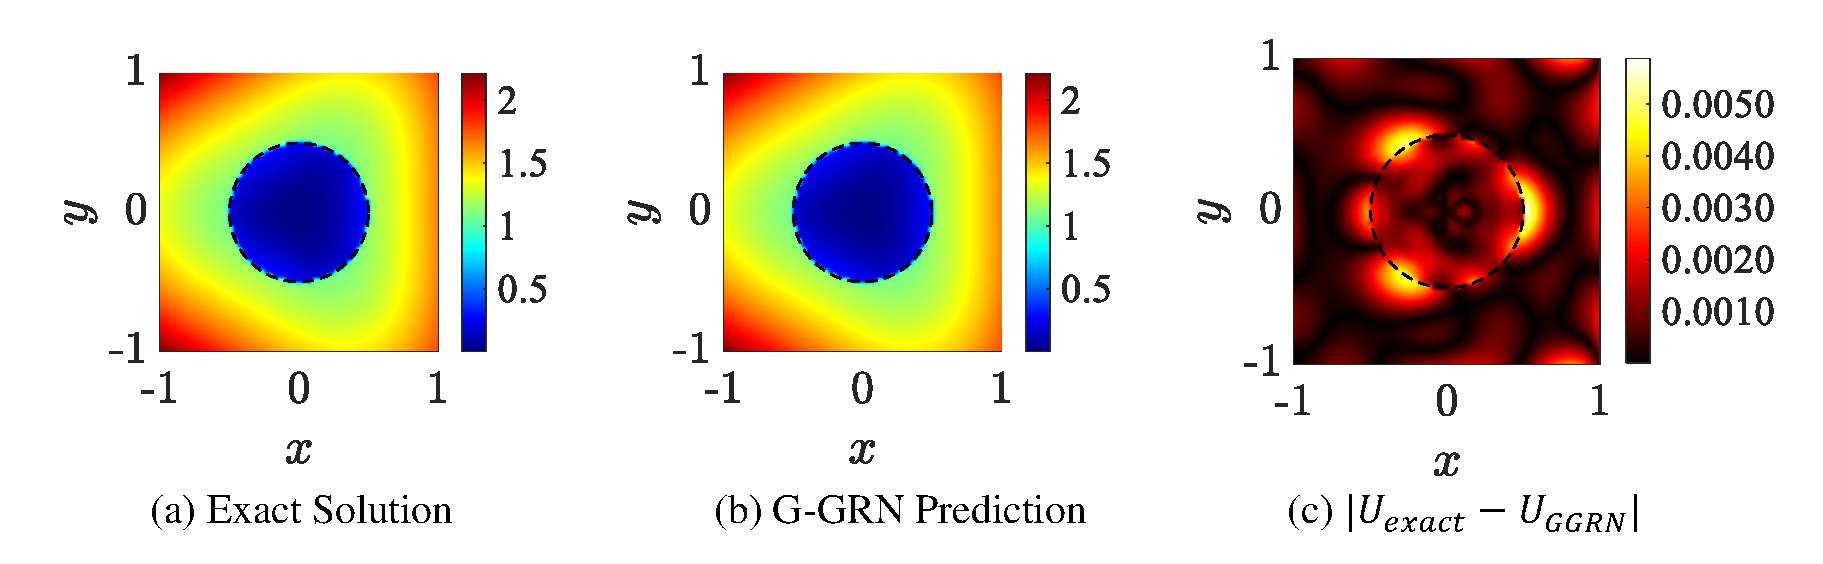
\includegraphics[width=\linewidth]{images/ex2.pdf}
    \caption{Example 2: Oscillating angular solution with $m=3$, $\varepsilon=0.3$, $\beta^-=1$, $\beta^+=10$, $N=64$. The dashed line indicates the interface $\Gamma$.}
    \label{fig:ex2_solution}
\end{figure}

\subsection{Example 3} \label{ex3}

Example \ref{ex3} replaces the circular interface with an ellipse $\Gamma: (x/a)^2 + (y/b)^2 = 1$ ($a = 0.6$, $b=0.4$, $\beta^- = 1$, $\beta^+ = 10$) to test G-GRN on an asymmetric geometry. Defining $\xi = (x/a)^2 + (y/b)^2$, we construct the exact solution as:
\begin{equation}
    u (\bf{x}) = \begin{cases}
        \xi, & \xi < 1, \\
        0.5 \xi + 0.625, & \xi >1.
    \end{cases}
\end{equation}
Because the outward normal of the ellipse varies continuously along the interface, this geometry imposes stricter requirements on the flux jump approximation $J_2 = [\beta \partial_n u]$ than the circular cases.

Figure \ref{fig:ex3_solution} displays the exact solution, the G-GRN prediction, and the pointwise absolute error at resolution $N=64$. The prediction preserves the gradient discontinuity across the elliptical interface, with an overall error level comparable to that of Example \ref{ex2}. The error heatmap (Figure \ref{fig:ex3_solution}c) shows that the maximum errors concentrate at the endpoints of the semi-major axis, where the curvature is largest; this pattern is consistent with the reduced accuracy of the midpoint normal approximation in high-curvature regions. At this resolution, the relative $L^2$ error is $1.88 \times 10^{-3}$. A joint convergence analysis of all three examples follows in Section \ref{subsec:conver}.

\begin{figure}[t]
    \centering
    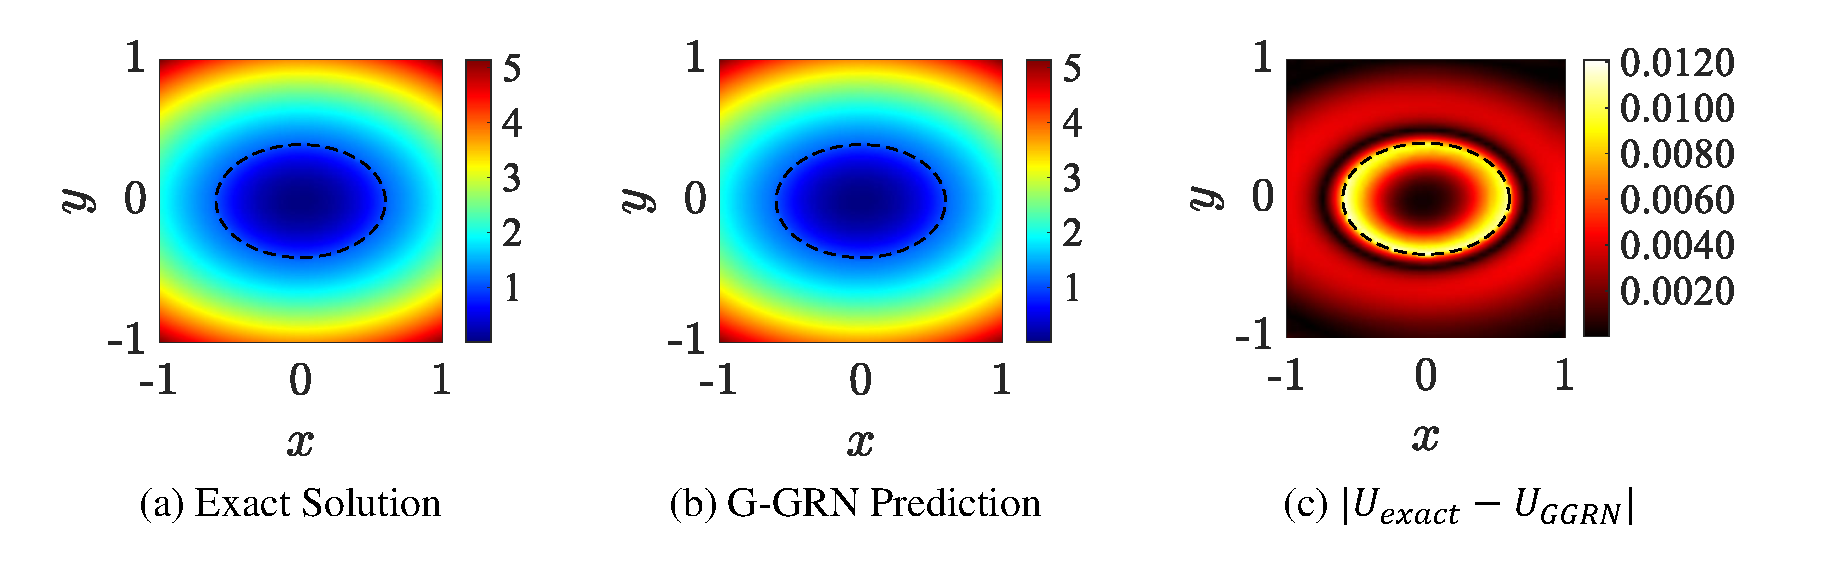
\includegraphics[width=\linewidth]{images/ex3.pdf}
    \caption{Example 3: Elliptic interface with $a=0.6$, $b=0.4$, $\beta^-=1$, $\beta^+=10$, $N=64$. The dashed line indicates the elliptic interface $\Gamma$.}
    \label{fig:ex3_solution}
\end{figure}

\subsection{Convergence study}
\label{subsec:conver}

Figure \ref{fig:2} summarizes the convergence behavior of all three test problems. Least-squares fits on the log-log data yield convergence orders of $p=0.54$ (Example \ref{ex1}), $p=0.45$ (Example \ref{ex2}), and $p=0.87$ (Example \ref{ex3}). All three cases exhibit a stable error reduction with increasing resolution. The highest rate is observed for Example \ref{ex3}, whose exact solution has the greatest regularity among the three test problems.

Figure \ref{fig:convergence_ggrn_pinn} compares the convergence of G-GRN and the standard PINN for Example \ref{ex1} ($\beta^- / \beta^+ = 1 / 10$). G-GRN achieves a convergence order of $p=0.54$, more than twice that of the PINN ($p = 0.24$). The gap is most pronounced between $N = 24$ and $N = 32$, where the PINN error stagnates ($e_{L^2}$: $1.41 \times 10^{-3} \to 1.42 \times 10^{-3}$) while G-GRN continues to reduce error monotonically. As discussed in Section \ref{sec:problem}, this sustained improvement reflects the higher fidelity of GFD stencil-based derivative approximations, which allow the network to translate finer grids into proportionally lower errors.

\begin{figure}
    \centering
    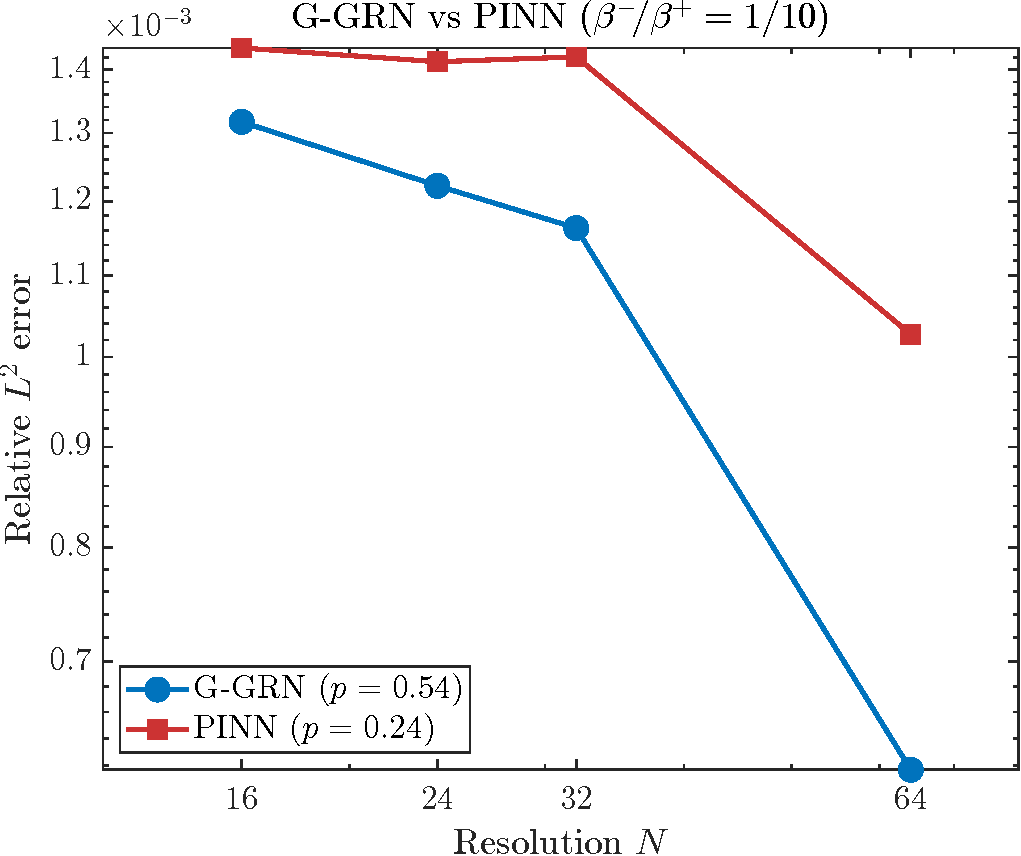
\includegraphics[width=0.5\linewidth]{images/convergence_ggrn_vs_pinn.pdf}
    \caption{Convergence comparison between G-GRN and PINN for the circular interface problem ($\beta^-/\beta^+=1/10$). The fitted slope $p$ indicates the convergence order.}
    \label{fig:convergence_ggrn_pinn}
\end{figure}

% ==================== Conclusion ====================
\section{Conclusion}
\label{sec:conclusion}

The central difficulty in applying neural networks to elliptic interface problems is that autograd-computed derivatives lose fidelity near coefficient discontinuities and fail to improve with grid refinement. G-GRN addresses this by delegating derivative computation to precomputed GFD stencils and restricting the network to learning the solution mapping, a separation that produces monotonic error reduction under mesh refinement where standard PINNs stagnate. Across three interface geometries (circular, oscillating, elliptic) with coefficient contrasts up to $1{:}100$, G-GRN reduces the relative $L^2$ error by $1.7\times$ and training time by $2.5\times$ over the PINN baseline at $N=64$, achieving a convergence order ($p=0.54$) more than twice that of the PINN ($p=0.24$). These results suggest that classical numerical stencils and graph neural networks are complementary rather than competing tools: the stencil encodes local differential structure that the network need not learn, while the network provides the nonlinear flexibility that fixed stencils lack. The current framework is restricted to 2D steady-state problems with known, static interfaces; extending G-GRN to three dimensions, time-dependent equations, and evolving geometries would test whether this complementarity holds in more demanding settings.

% ---------- Bibliography ----------
\bibliographystyle{plainnat}  % or unsrtnat
\bibliography{reference}

\end{document}
